%
%  Chris Thoma
%
\documentclass[12pt,fullpage]{article}
\usepackage{fullpage}
\usepackage{psfrag}                                          % LaTeX graphics tool
\usepackage{pslatex}                                         % avoids the default cmr font
\usepackage{graphicx}                                        % graphics package 
\usepackage{epsfig}
\usepackage{hyperref}
\usepackage{color}

\begin{document}

\noindent
{\bf Weibull distribution} (from \color{blue}\url{http://www.math.wm.edu/~leemis/chart/UDR/UDR.html}\color{black})

\noindent
The shorthand $X \sim \hbox{Weibull}(\alpha, \, \beta)$ is used to indicate that the
random variable~$X$ has the Weibull distribution with scale parameter $\alpha > 0$ and shape parameter $\beta > 0$.
A Weibull random variable $X$ has probability density function 
$$
f(x) = \frac{\beta}{\alpha} \kern 0.04em x ^ {\kern 0.04em \beta - 1} e ^ {- (1/ \alpha) x ^ {\kern 0.04em \beta}} \qquad \qquad x > 0.
$$
The Weibull distribution is used in reliability and survival analysis to model the lifetime of an object, the lifetime of a organism, or a service time.
The accelerated life and Cox proportional hazards model are identical when the baseline distribution is Weibull.
The probability density function is plotted below for $\alpha = 1$ and $\beta = 1/2, \, 1, \, 2, \, 3$.

\begin{figure}[h!]
\begin{center}
\psfrag{labx}{$x$}
\psfrag{labf}{$f(x)$}
\psfrag{lab1}{$\beta \kern -0.08em = \kern -0.08em 1$}
\psfrag{lab2}{$\beta \kern -0.08em = \kern -0.08em 2$}
\psfrag{lab3}{$\beta \kern -0.08em = \kern -0.08em 3$}
\psfrag{lab5}{$\beta \kern -0.08em = \kern -0.08em 1/2$}
\includegraphics[width=3.2in]{WeibullPlot.ps}
\end{center}
\end{figure}

\noindent
The cumulative distribution function on
the support of $X$ is
$$
F(x) = P(X \le x) = 1 -  e ^ {- (1 /\alpha) x^ {\kern 0.04em \beta}} \qquad \qquad x > 0.
$$
The survivor function on the support of $X$ is
$$
S(x) = P(X \ge x) = e ^ {- (1 /\alpha) x^{\kern 0.04em \beta}} \qquad \qquad x > 0.
$$
The hazard function on the support of $X$ is
$$
h(x) = \frac{f(x)}{S(x)} = \frac{\beta}{\alpha} \kern 0.04em  x ^ {\kern 0.04em \beta-1} \qquad \qquad x > 0.
$$
The cumulative hazard function on the support of $X$ is
$$
H(x) = - \ln S(x) = \frac{1}{\alpha} \kern 0.04em  x ^ {\kern 0.04em \beta} \qquad \qquad x > 0.
$$
The inverse distribution function of $X$ is
$$
F ^ {-1}(u) = \left[ - \alpha \ln (1 - u) \right] ^ {1 / \beta} \qquad \qquad 0 < u < 1.
$$
The median of $X$ is
$$
(\alpha \, \ln 2)^{1 / \beta}.
$$
The moment generating function of $X$ is
$$
M(t) = E\left[ e ^ {\kern 0.04em tX} \right] =
\displaystyle \int_0 ^\infty e^{tx}
\frac{\beta}{\alpha} \kern 0.04em x ^ {\kern 0.04em \beta - 1}
e ^ {- (1/ \alpha) x ^ {\kern 0.04em \beta}}
\, dx \qquad \qquad t > 0.
$$
The characteristic function of $X$ is
$$
\phi(t) = E\left[ e ^ {itX} \right] = \displaystyle \int_0 ^\infty e^{itx} \frac{\beta}{\alpha} \kern 0.04em x ^ {\kern 0.04em \beta - 1} e ^ {- (1/ \alpha) x ^ {\kern 0.04em \beta}} \, dx \qquad \qquad t > 0.
$$
The population mean, variance, skewness, and kurtosis of $X$ are
$$
E[X] = \frac{\alpha}{\beta} \Gamma \left( \frac{1}{\beta} \right) \qquad \qquad 
V[X] = \alpha^2 \left\{ \frac{2}{\beta} \Gamma \left( \frac{2}{\beta} \right) - \left[ \frac{1}{\beta} \Gamma \left( \frac{1}{\beta} \right) \right]^2 \right\} \qquad \qquad 
$$
$$
E\left[ \left( \frac{X - \mu}{\sigma} \right) ^ 3 \right] = \left\{ \frac{2}{\beta} \Gamma \left( \frac{2}{\beta} \right) - \left[ \frac{1}{\beta} \Gamma \left( \frac{1}{\beta} \right) \right]^2 \right\}^{-3/2} \left\{ \frac{3}{\beta} \Gamma \left( \frac{3}{\beta} \right) - \frac{6}{\beta^2} \Gamma \left( \frac{1}{\beta} \right) \Gamma \left( \frac{2}{\beta} \right) + 2 \left[ \frac{1}{\beta} \Gamma \left( \frac{1}{\beta} \right) \right]^3 \right\}
$$
\begin{small}
$$
E\left[ \left( \frac{X - \mu}{\sigma} \right) ^ 4 \right] = \left\{ \frac{2}{\beta} \Gamma \left( \frac{2}{\beta} \right) - \left[ \frac{1}{\beta} \Gamma \left( \frac{1}{\beta} \right) \right]^2 \right\}^{-2} \left\{ \frac{4}{\beta} \Gamma \left( \frac{4}{\beta} \right) - \frac{12}{\beta^2} \Gamma \left( \frac{1}{\beta} \right) \Gamma \left( \frac{3}{\beta} \right) \right.
$$
\end{small}

\vspace{-0.1 in}

\begin{small}
$$
\left.
+ \frac {12}{\beta^3} \left[ \Gamma \left( \frac{1}{\beta} \right) \right]^2 \Gamma \left( \frac{2}{\beta} \right) - \frac{3}{\beta^4}
\left[ \Gamma \left(\frac{1}{\beta}\right)\right]^4 \right\}.
$$
\end{small}
%   For $X_1, \, X_2, \, \ldots , \, X_n$ mutually independent Weibull($\alpha$) random variables,
%   the maximum likelihood estimator for $\alpha$ is
%   $$
%   \hat \alpha = \left(\frac{\sum_{i\,=\,1}^n X_i}{n}\right)^{1 / \hat\beta}.
%   $$

\vspace{0.1in}

\noindent
{\bf APPL verification:}
The APPL statements
\begin{verbatim}
X := WeibullRV(1 / alpha, beta);
CDF(X);
HF(X);
IDF(X);
Mean(X);
Variance(X);
Skewness(X);
Kurtosis(X);
MGF(X);
\end{verbatim}
verify the cumulative distribution function, hazard function, population mean, variance, skewness, kurtosis, and moment generating function.
\end{document}
